%% PREAMBLE
% Specify document class:
\documentclass[12pt]{article}

% Load in packages:
\usepackage[utf8]{inputenc}
\usepackage[margin=1in]{geometry}
% These are popular math-writing packages
\usepackage{amsmath}
\usepackage{mathrsfs}
\usepackage{amssymb}
\usepackage{mathtools}
\usepackage{bbm}
\usepackage{tabularx}  % For flexible tables
\usepackage{booktabs}  % For professional-looking horizontal lines
\usepackage{caption}   % For table captions
\usepackage{graphicx}   % For inserting images
\usepackage{caption}    % For captions
\usepackage{float}      % For precise control over figure placement
\usepackage{parskip}
\usepackage{dcolumn}

%\setlength{\parindent}{10ex}
\usepackage{graphicx}
\usepackage{xcolor}
\usepackage{hyperref}

\usepackage[backend=biber,style=apa,natbib]{biblatex} 
\addbibresource{memo/bib.bib} 

%% FRONT MATTER
\title{The Broad Center Superintendent Research Dataset \\  V1: September 5th, 2025}
\date{}
\begin{document}

\maketitle
\section{Overview}
This document contains figures and tables generated using the Superintendent Research Dataset. 

The data described here are in the file \textbf{\texttt{data/processed/combined\_superintendents.csv}}. All figures and tables are produced in \textbf{\texttt{03\_tables\_figures.R}} and can be found in the folder \textbf{\texttt{/scripts}}. See the README file for details on data generation. 

You are welcome to use these data. Please do so with the following citation: 

\noindent Stemper, Sam and The Broad Center. Superintendent Research Dataset (v1, 2025-09-05), 2025. 

Statistics may differ somewhat from \citet{stemper} due to updates in the dataset. 

\section{Coverage}
The dataset includes records for 20 states. Figure \ref{fig:state_years_plot} displays years of coverage and data types available for each state. Figures \ref{tab:district_counts_by_state_year} and \ref{tab:balanced_district_counts_by_state_year} report, respectively, the number of districts for which we have data in each state-year combination and the number of districts for which we have a balanced panel of data across all available state-years. 

Figure \ref{fig:student_coverage_by_year} displays the ratio of total enrollment in districts for which we have data to total public school enrollment in a) covered state-years, and b) the US as a whole. In the state-years where we have data, coverage is nearly complete. Our data cover a majority of US school enrollment from 2010-2022. For example, as reported in Table \ref{tab:superintendent_coverage_enrollment_2014}, in 2014, covered districts account for 61\% of public school enrollment and 68.8\% of school districts in the US. 

\section{Benchmarking}

We benchmark descriptive statistics in our data to published results. 

We first consider superintendent turnover. We compute turnover using our superintendent identifiers, which are created by matching superintendents on name within states. Figure \ref{fig:superintendent_turnover_overall}  reports turnover rates for each year. 

Table \ref{tab:white_turnover_table} compares our estimated turnover rates for the years 2020-2022 to those reported by \citet{white} at the national level. Though the samples are different (\citet{white} uses national data and we use data from the states in our sample), our estimates are similar.  

We next consider superintendent gender. We code superintendent gender on the basis of names. Table \ref{tab:superintendent_demographics} reports state-by-state comparisons to \citet{superintendentlab}. An exact comparison is not possible here because \citet{superintendentlab} reports results for 2024-25 and our data go through 2023-24. However, overall levels are similar. 

\section{Known issues}

\subsection{Turnover rates}
Figure \ref{fig:superintendent_turnover_by_state_year} reports turnover estimates by state and year. There are some state-year combinations where turnover rates are non-missing but very low. For example,  New York in 2017 or Oklahoma 2020 fit this description. This is likely because the data snapshots used to construct superintendent rosters in those state-year cells come from nearby months  within consecutive academic years. 

\subsection{Salaries}
Some reported salary values are implausibly low for full-year superintendent positions. We keep these values in the dataset for transparency but note that entries of 0 or very low salaries in some states may not reflect actual full-year compensation.


\section*{Figures}
\begin{figure}[H]
\caption{Data coverage}
    \label{fig:state_years_plot}
    \centering
    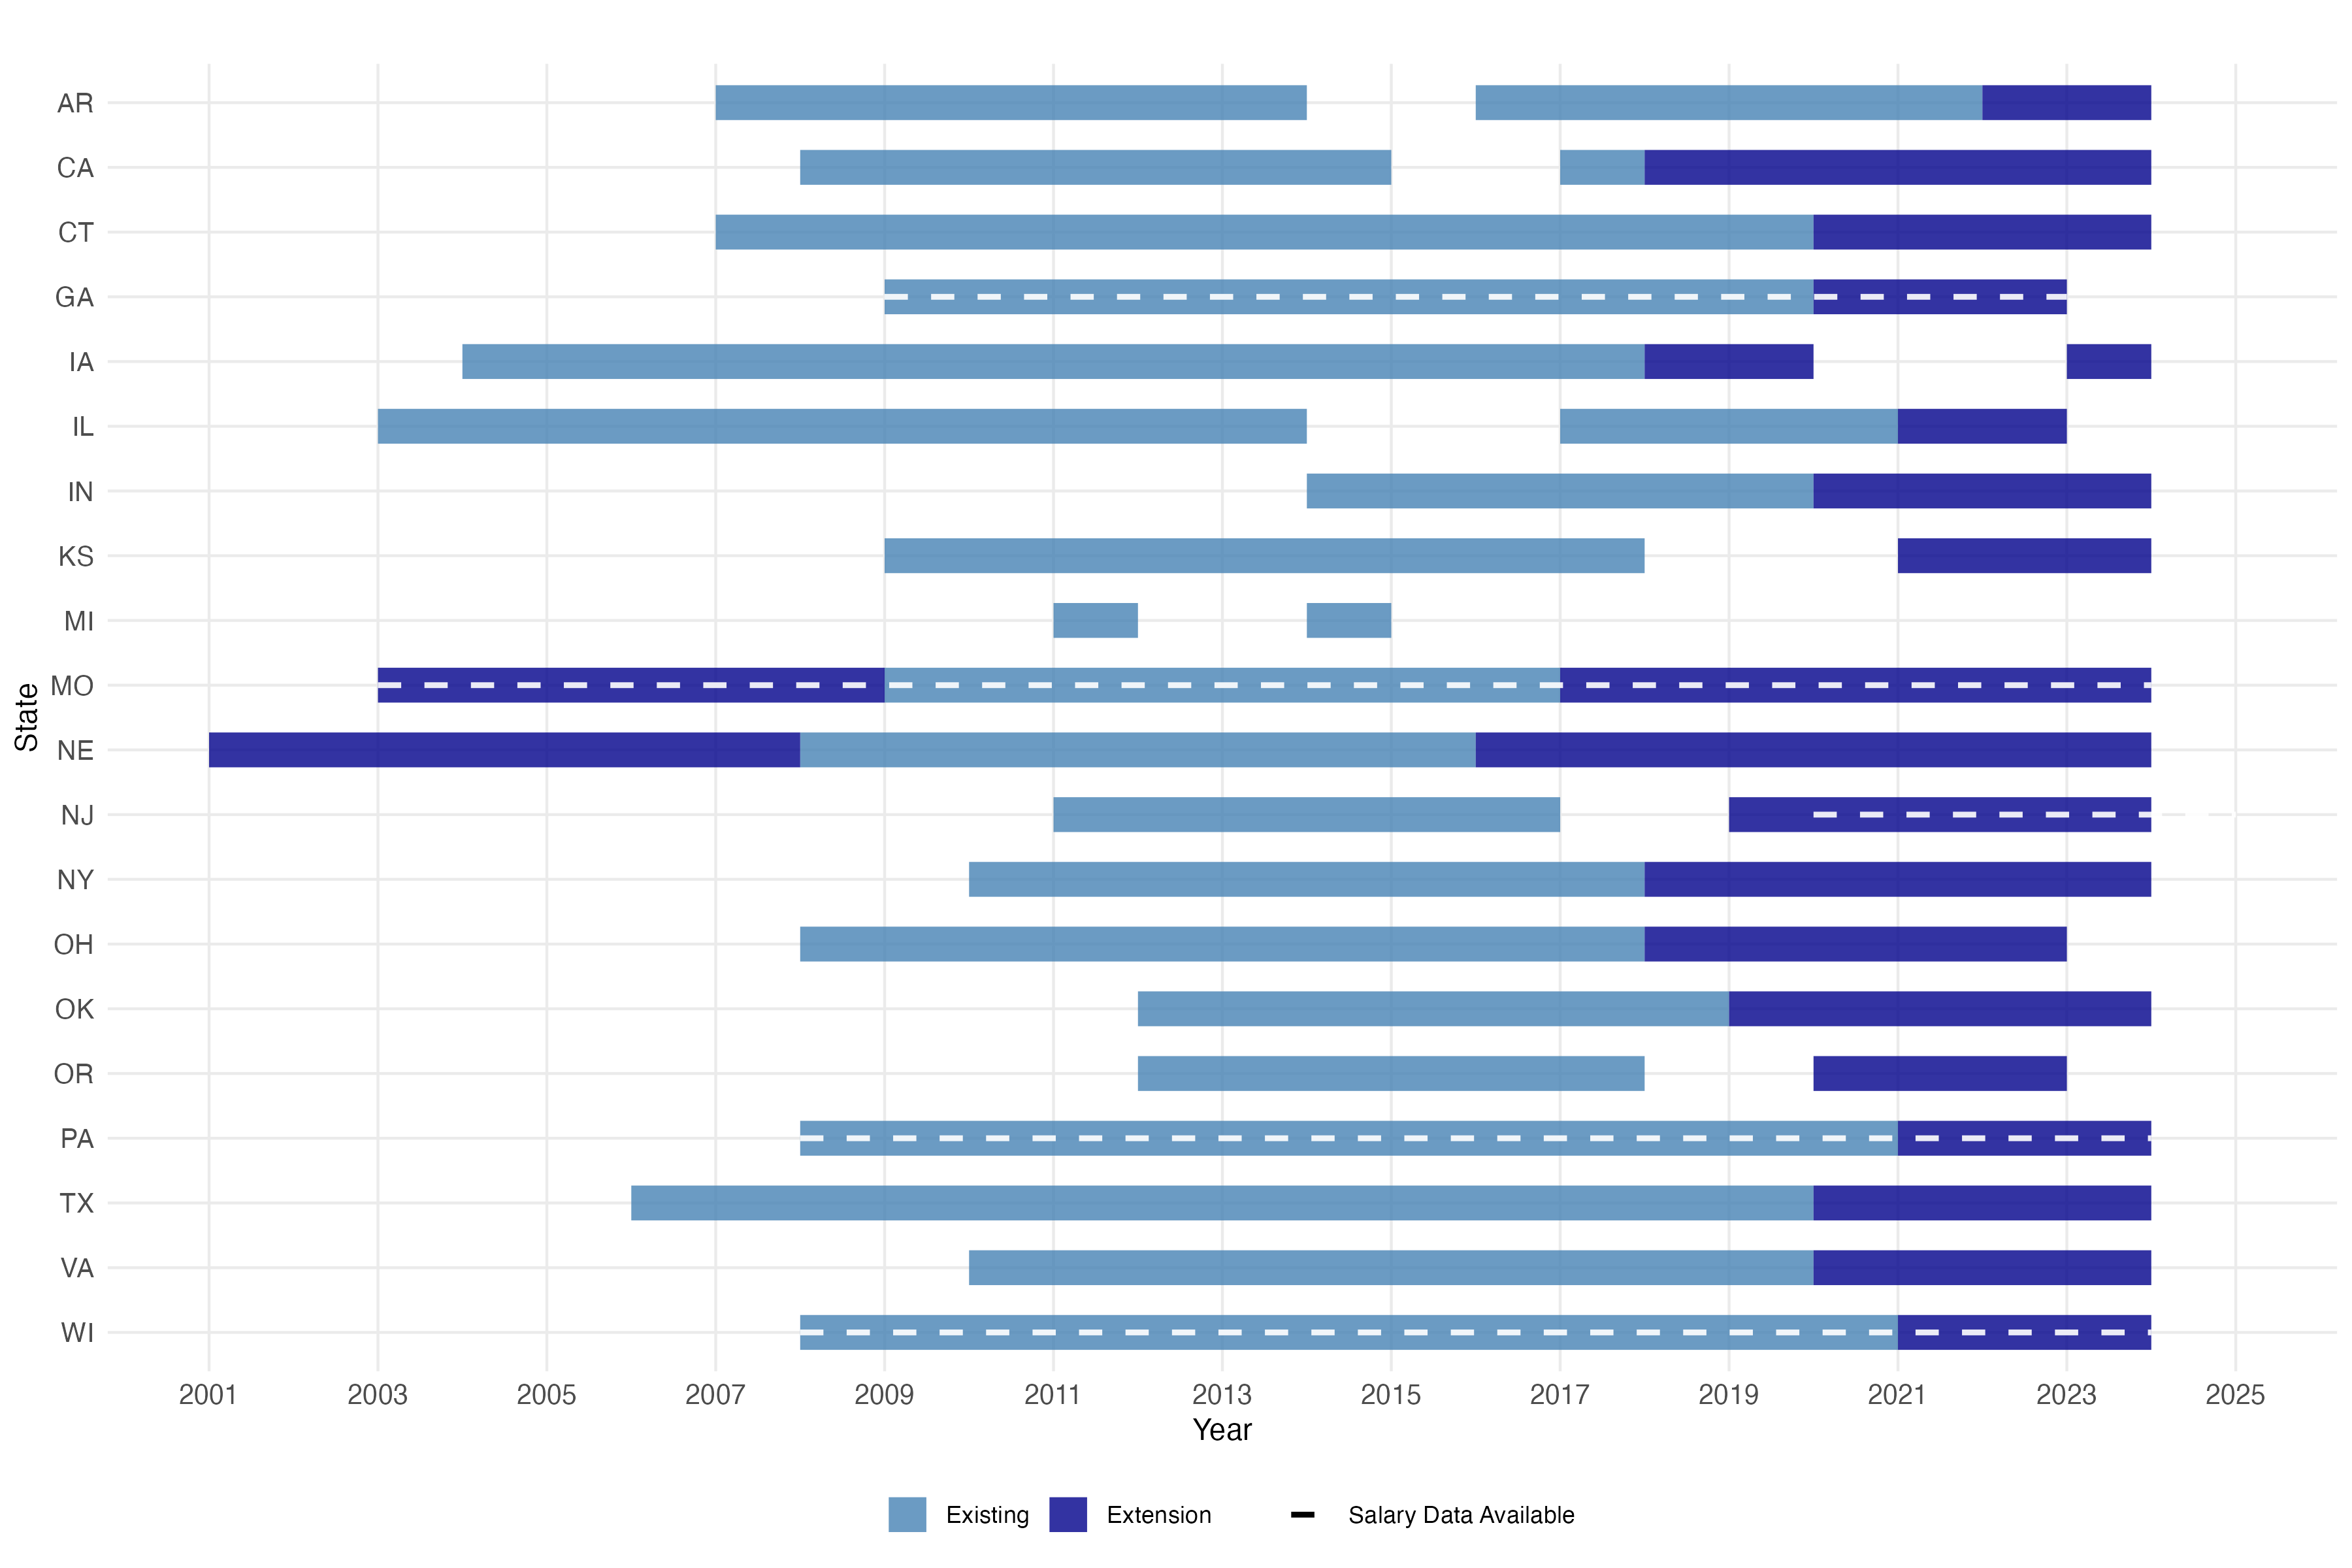
\includegraphics[width=0.9\textwidth]{figures/state_years_plot.png}
    \caption*{\footnotesize Notes: Year refers to the fall of the academic year. ``Existing'' data are those used in \citet{stemper}. }
\end{figure}


\begin{figure}[H]
\caption{District counts by state and year}
    \label{tab:district_counts_by_state_year}
    \centering
    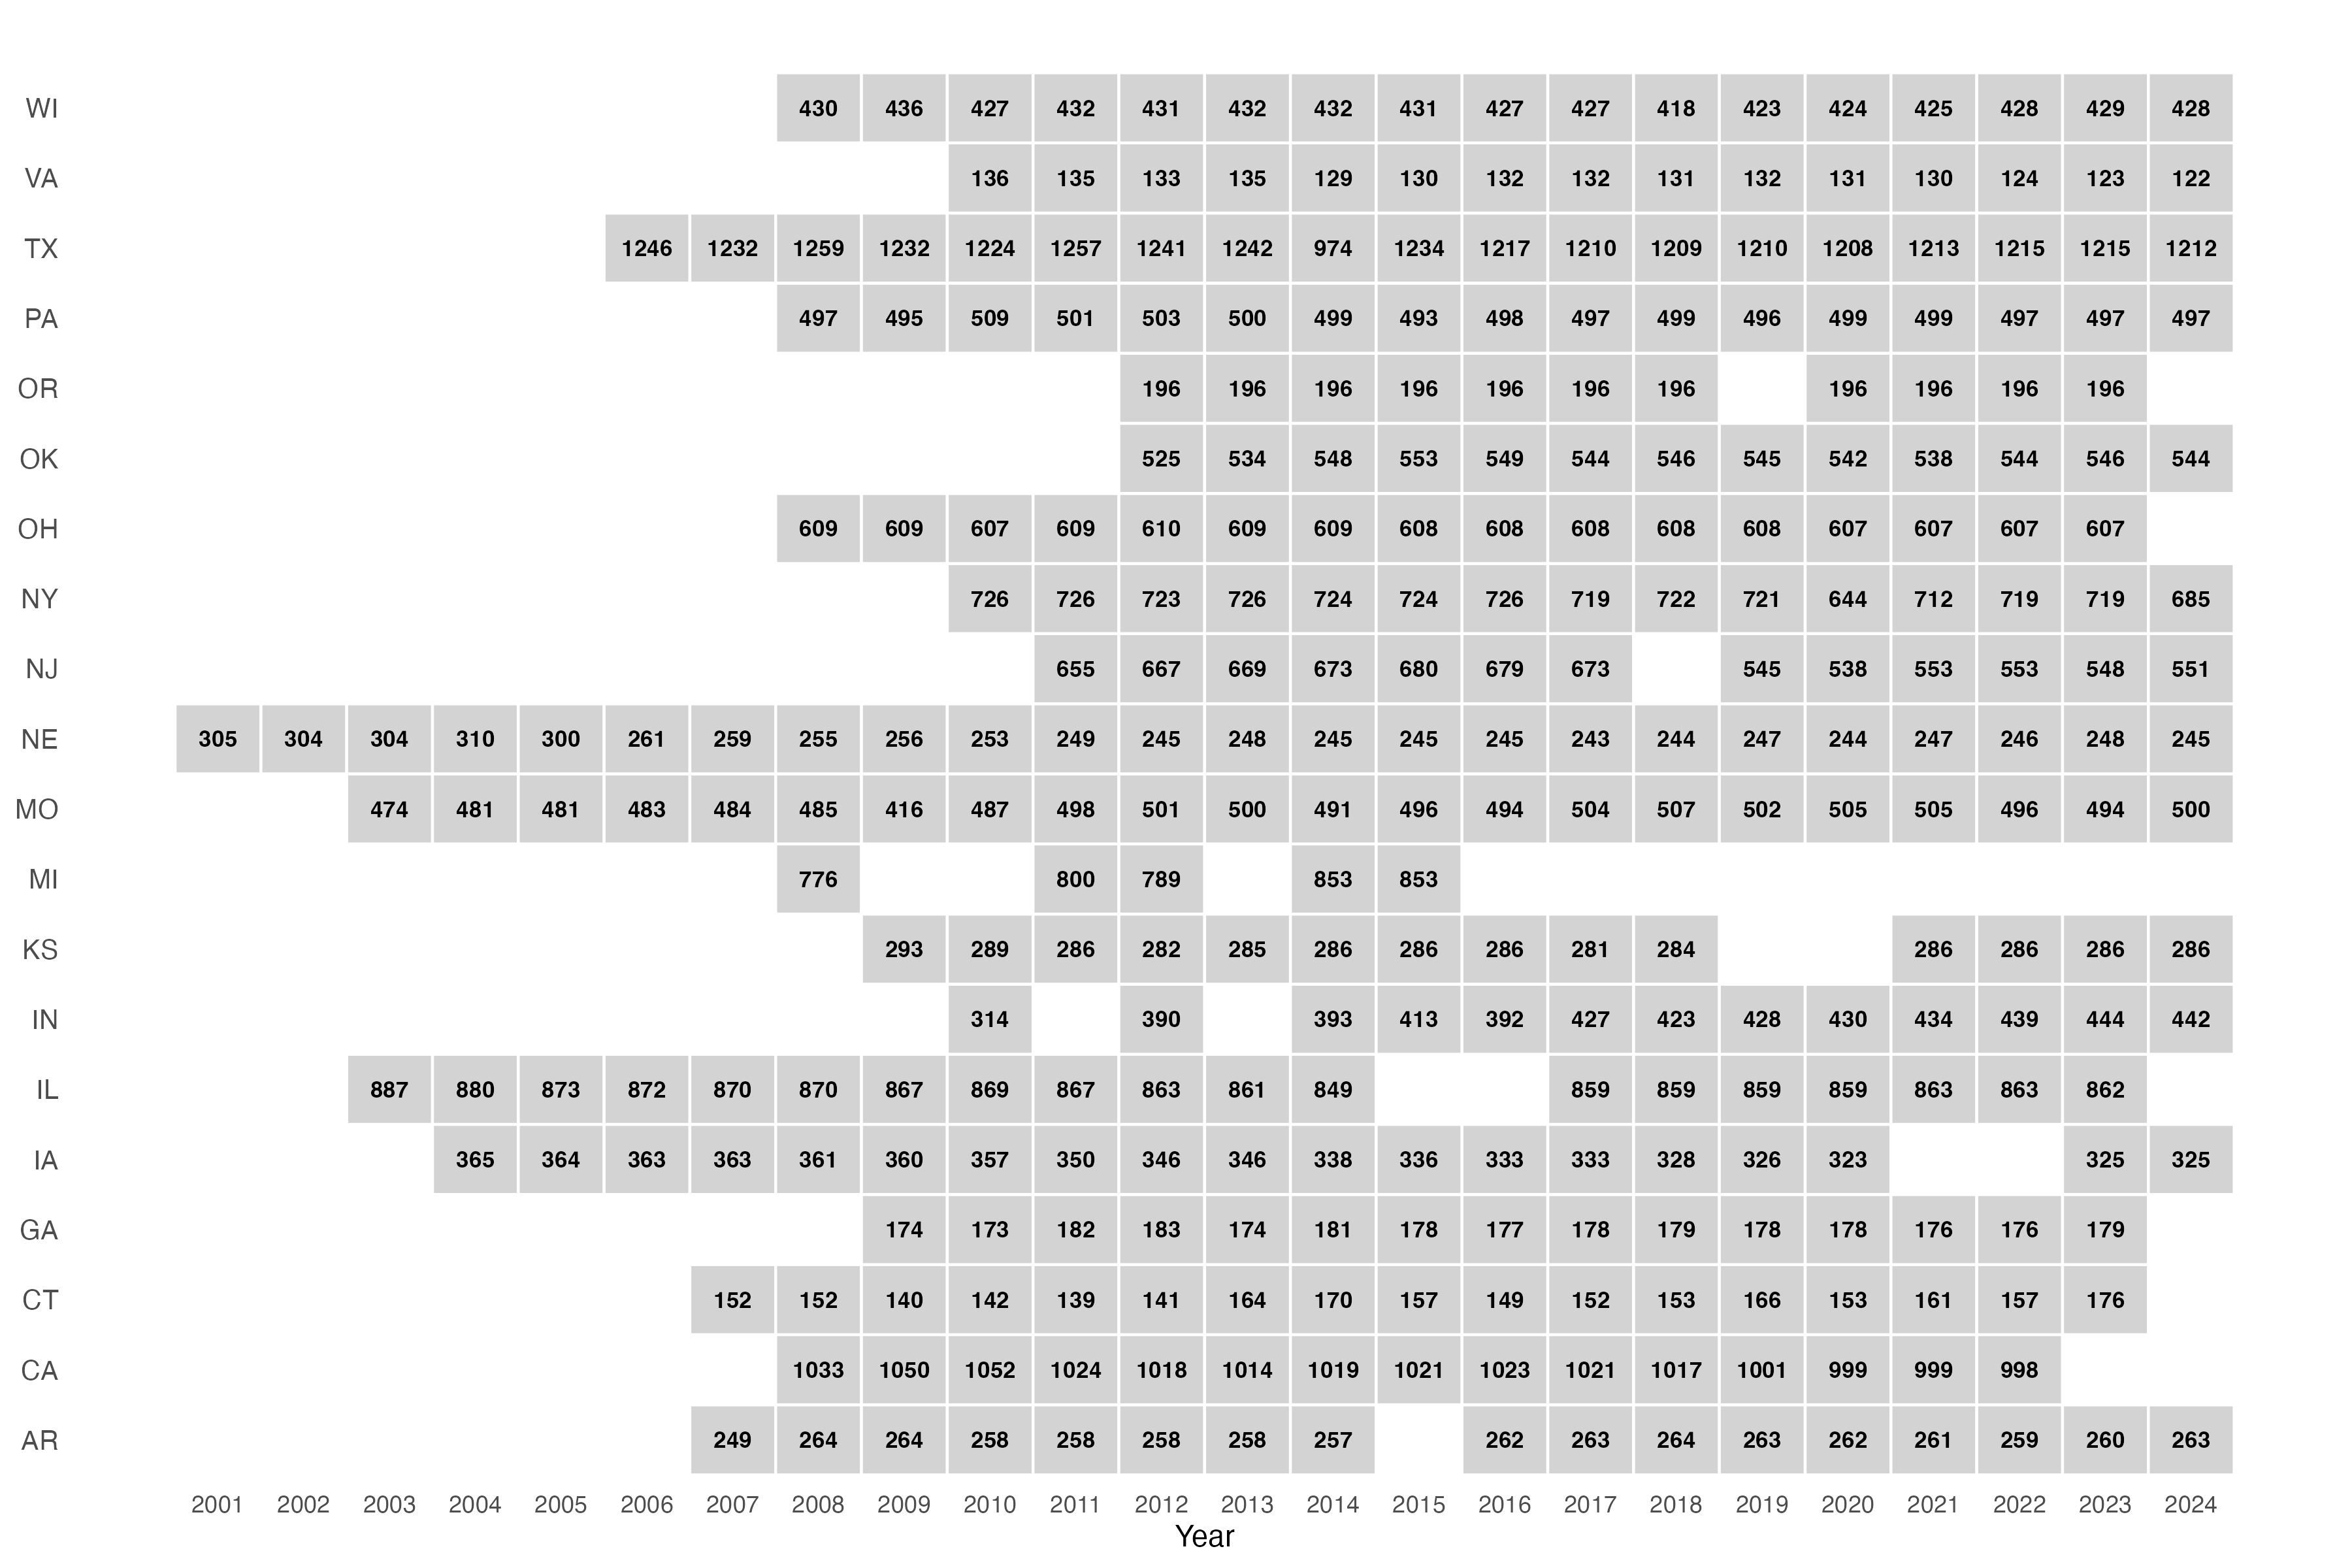
\includegraphics[width=0.8\textwidth]{figures/district_counts_by_state_year.png}
     \caption*{\footnotesize Notes: This figure shows the number of districts for which superintendents data is available.}
\end{figure}

\begin{figure}[H]
    \caption{Balanced district counts by state and year}
    \label{tab:balanced_district_counts_by_state_year}
    \centering
    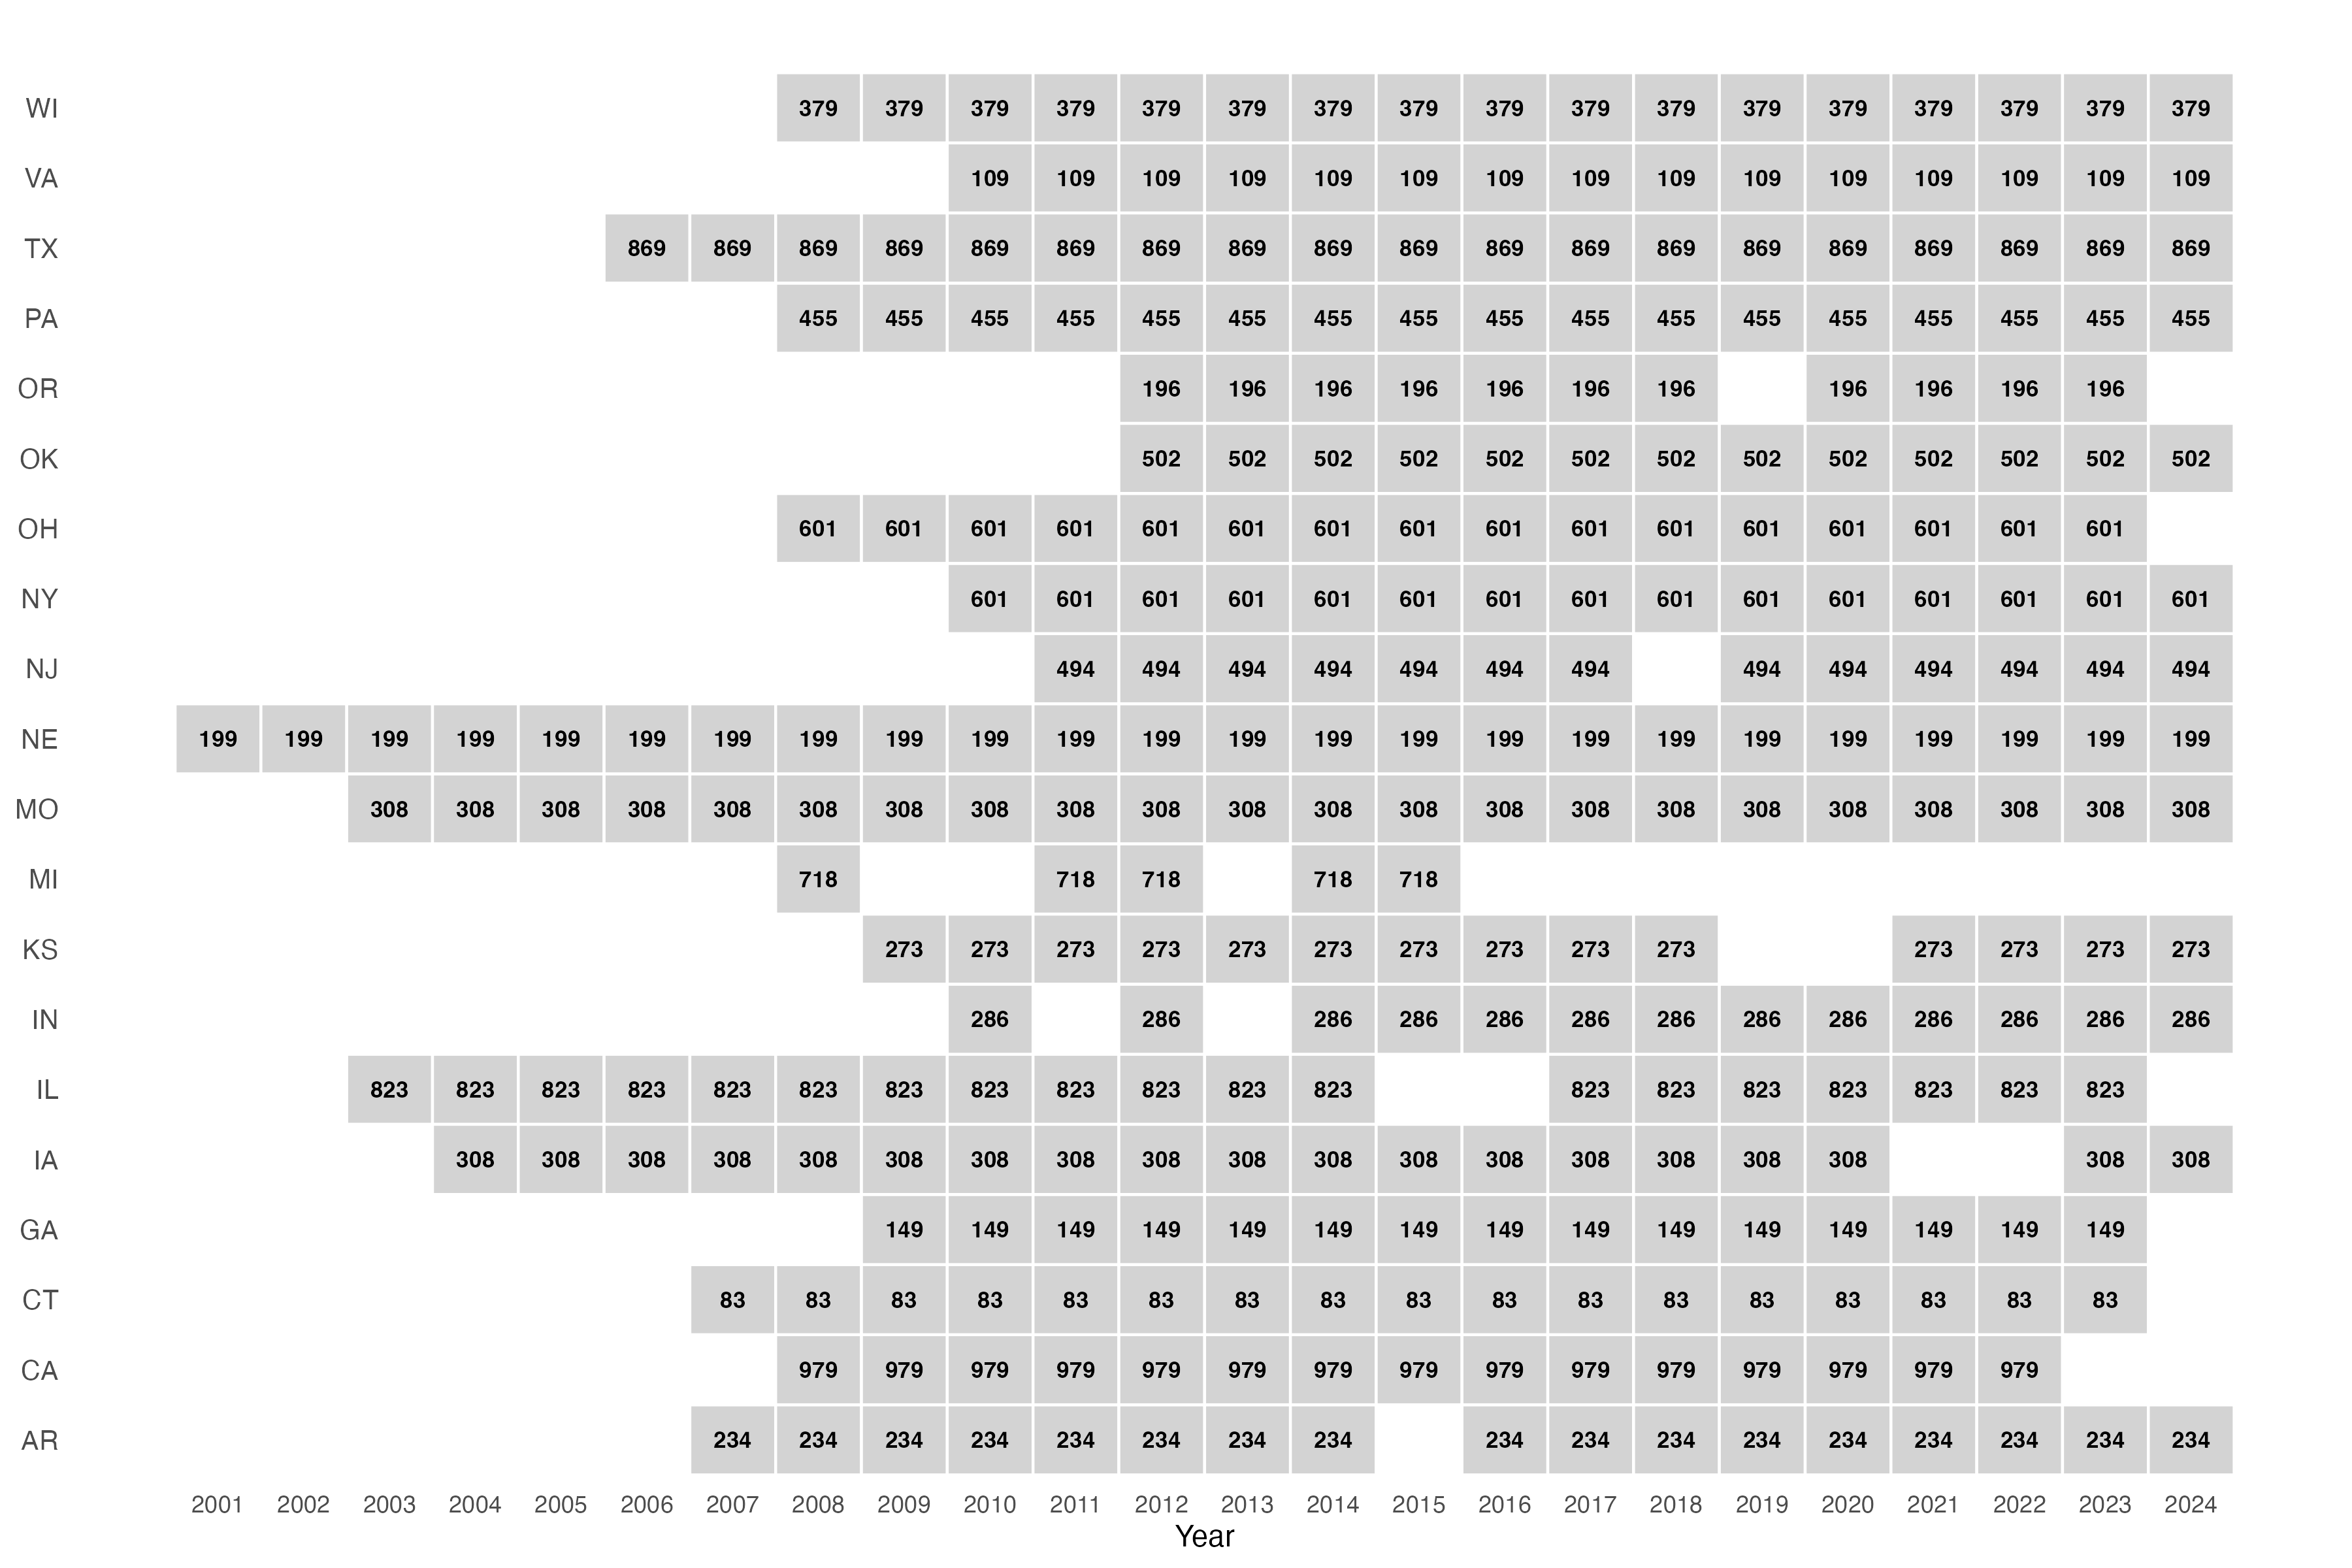
\includegraphics[width=0.8\textwidth]{figures/balanced_district_counts_by_state_year.png}
     \caption*{\footnotesize Notes: This figure shows the number of districts for which superintendents data is available in every year for which we have data for that state.}
\end{figure}

\begin{figure}[H]
    \caption{Enrollment coverage by year}
    \label{fig:student_coverage_by_year}
    \centering
    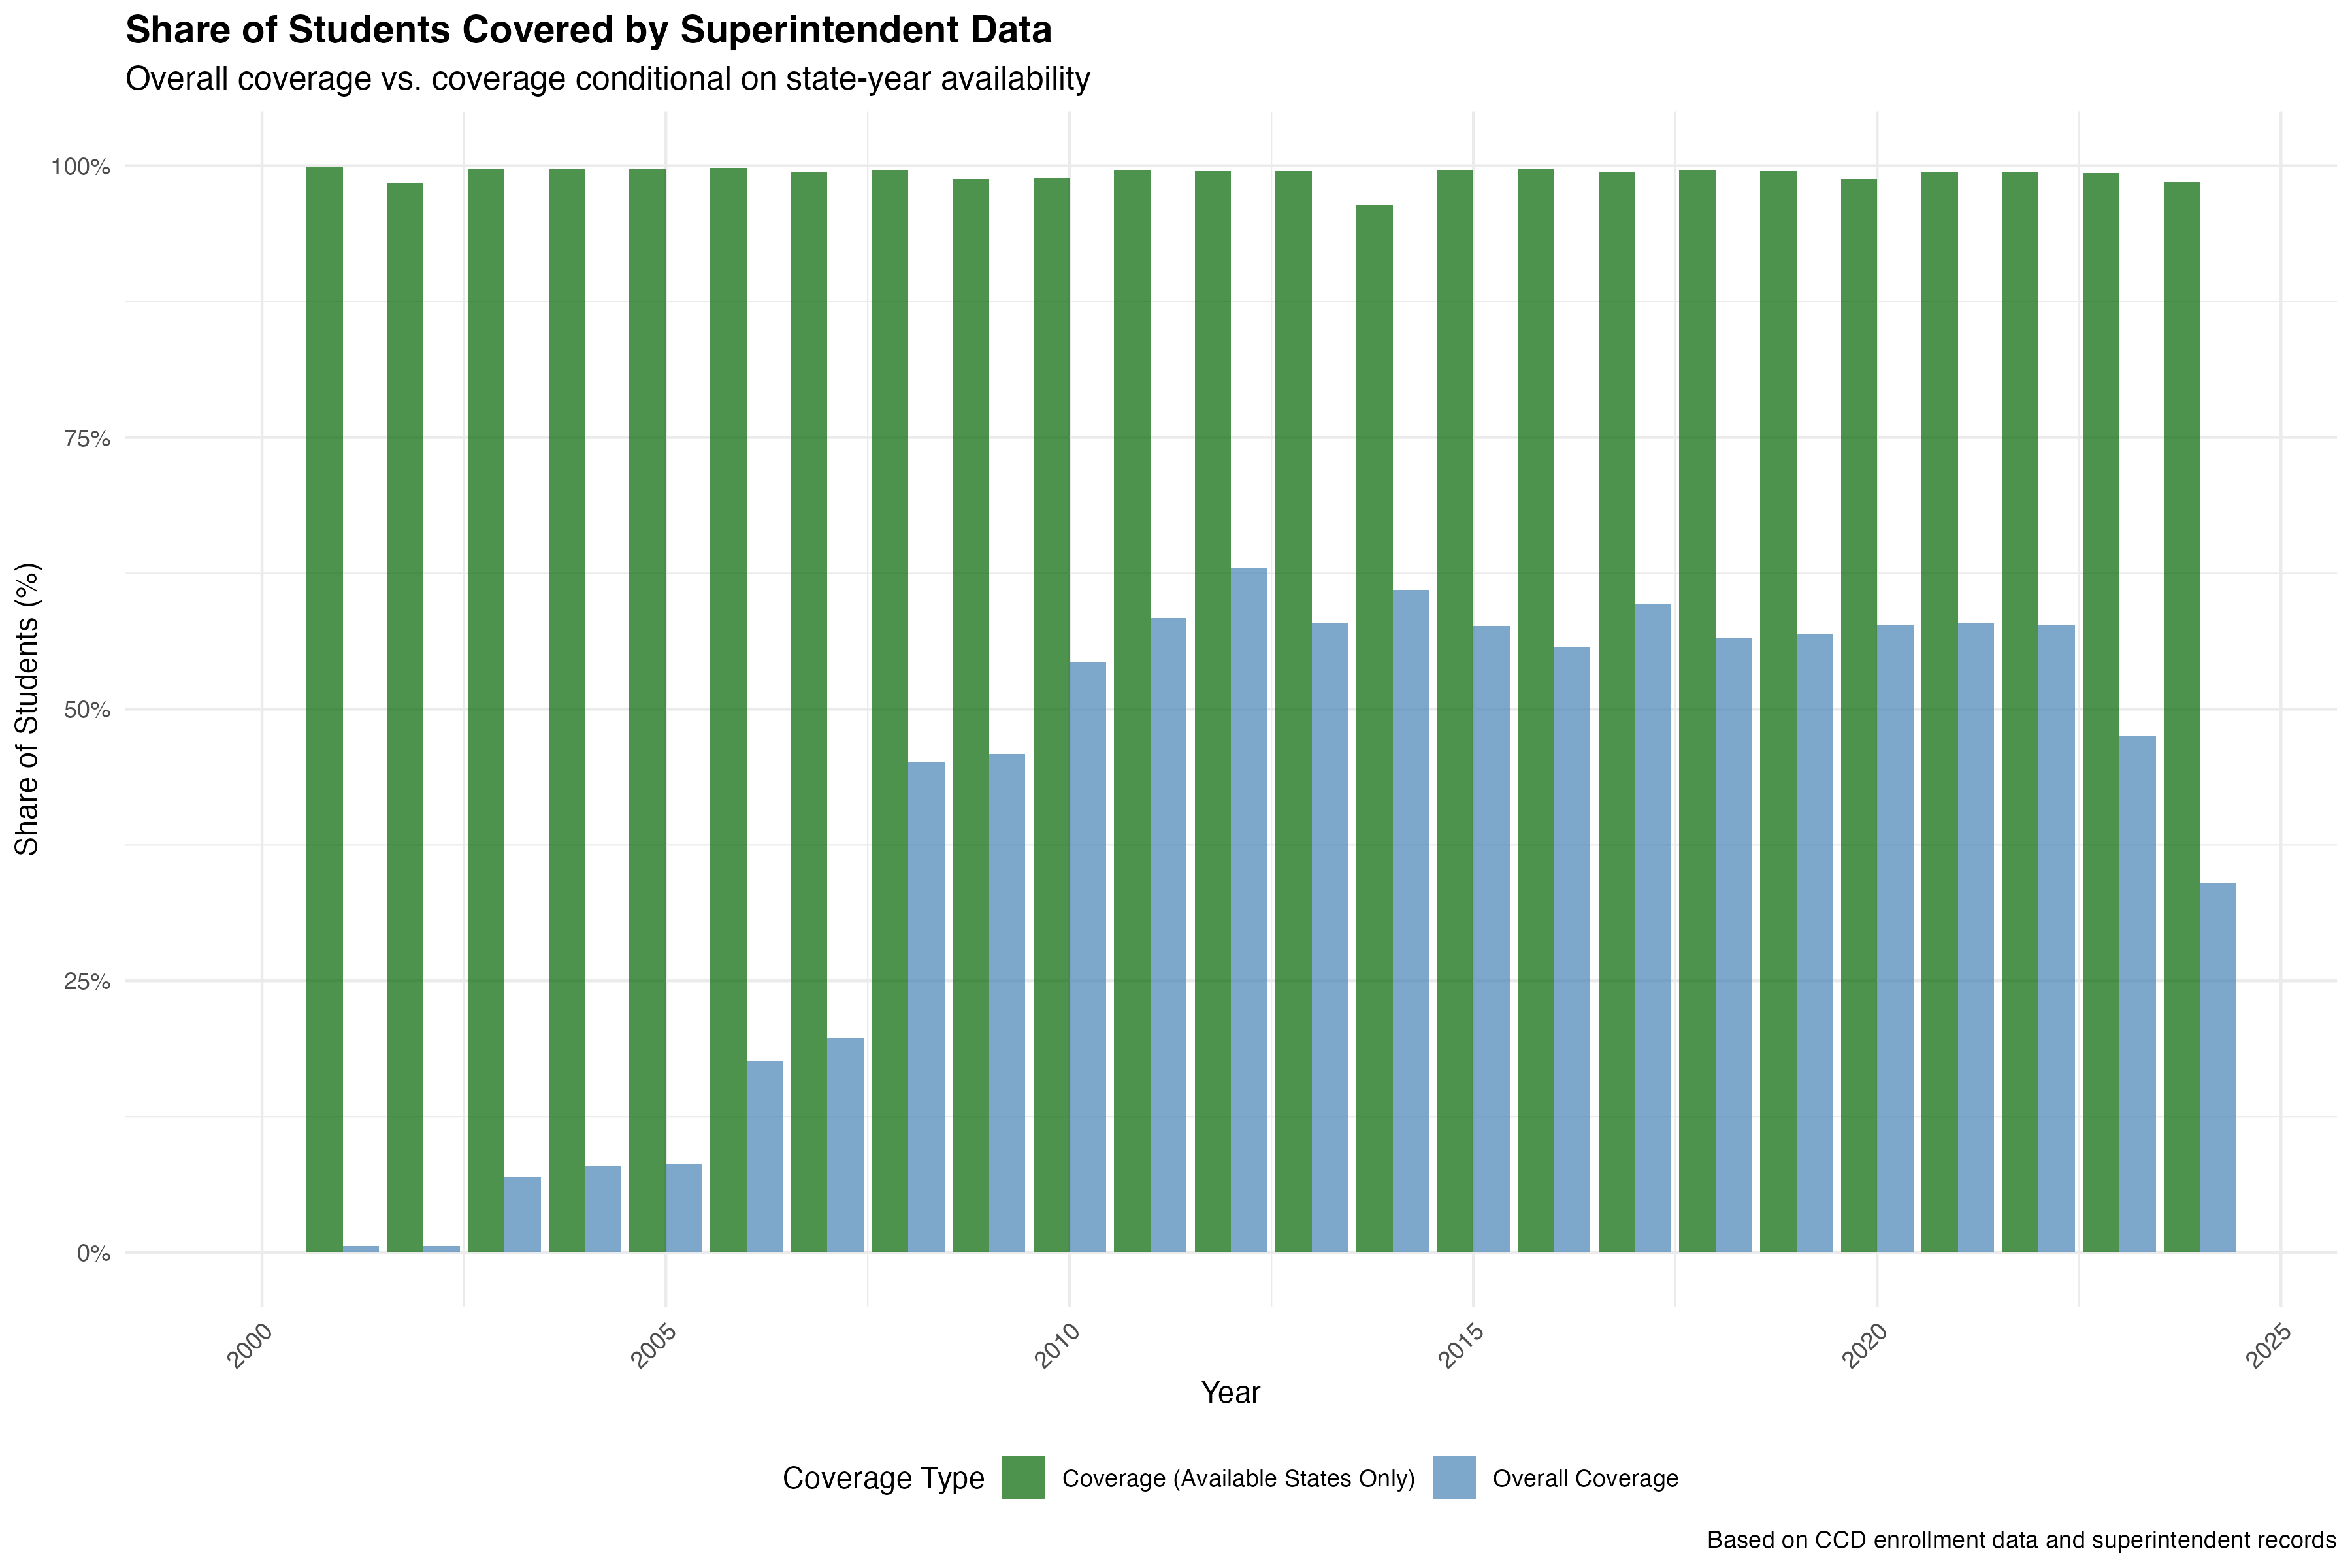
\includegraphics[width=0.9\textwidth]{figures/student_coverage_by_year.png}
     \caption*{\footnotesize Notes: This figure shows the share of students covered in our data in the country overall (blue bars) and in states for which we have superintendents data in that year (green bars). Coverage is calculated by dividing the student enrollment counts in regular public school districts in our data by total enrollment in regular public school districts. Enrollment data come from the Common Core of Data (CCD). Districts not labeled as ``regular public school district[s]'' by the CCD are excluded from these calculations.}
\end{figure}

\begin{figure}[H]
    \caption{Superintendent turnover by year}
    \label{fig:superintendent_turnover_overall}
    \centering
    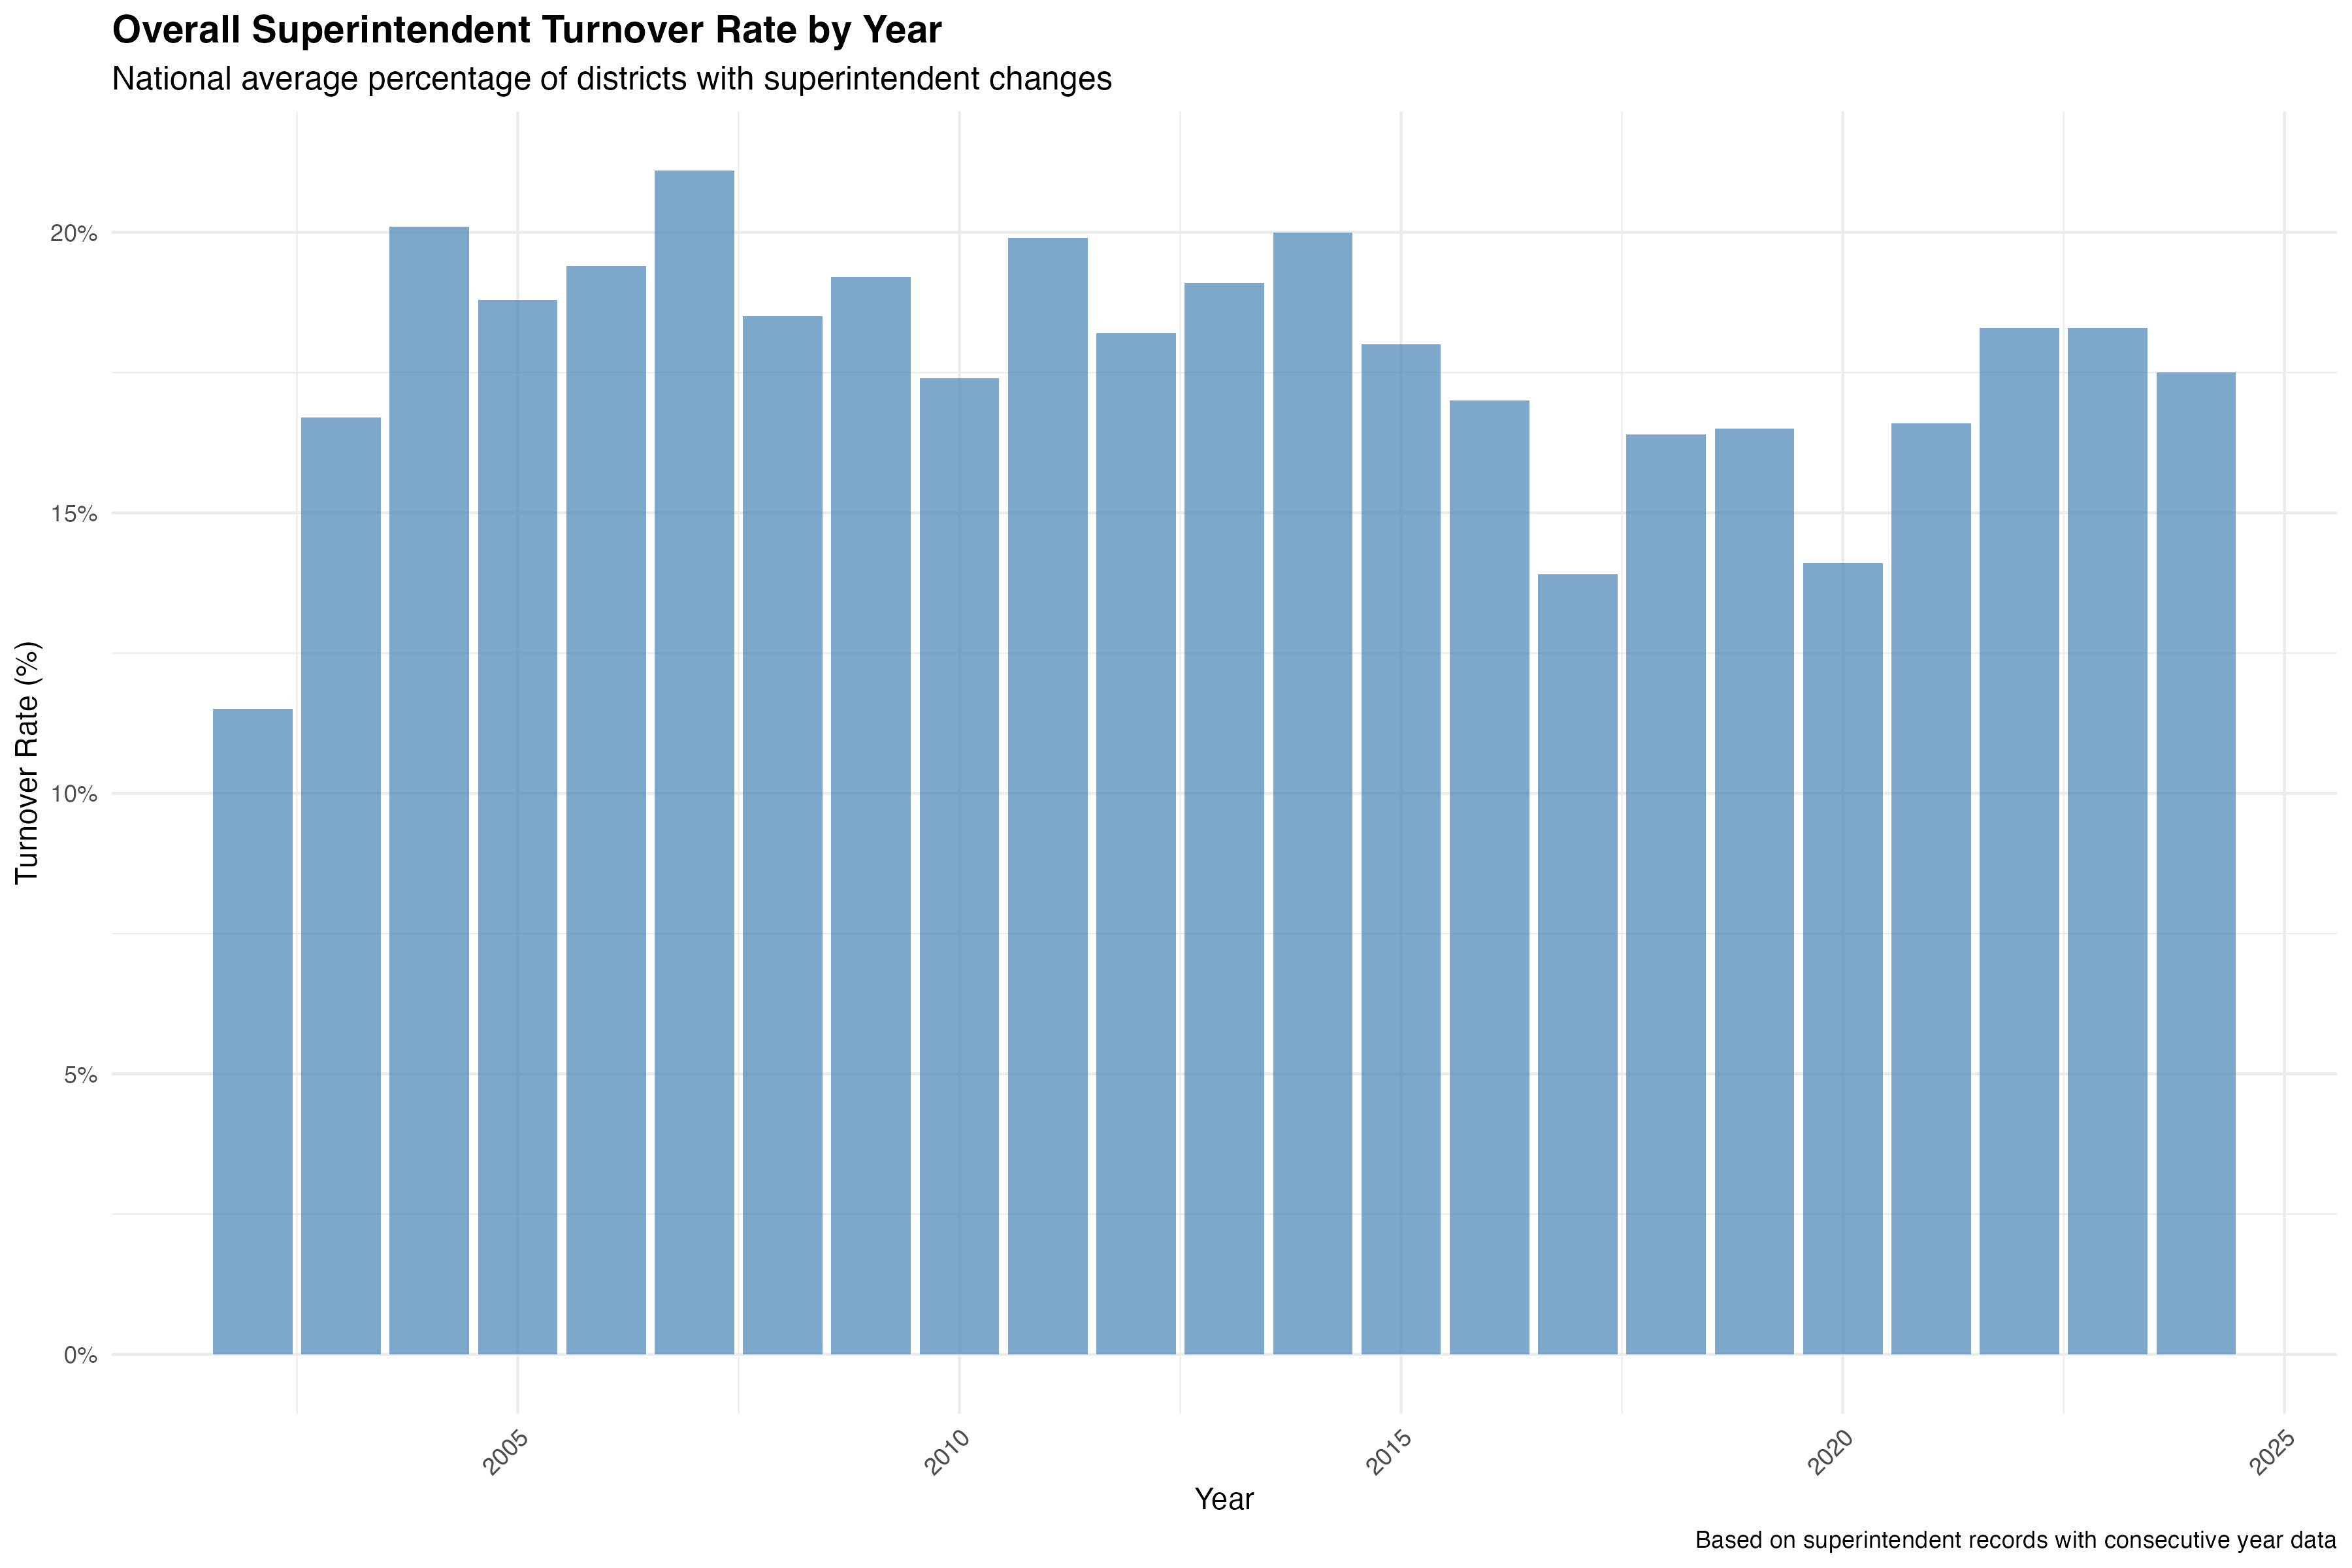
\includegraphics[width=0.9\textwidth]{figures/superintendent_turnover_overall.png}
    \caption*{\footnotesize Notes: A district is considered to have a superintendent turnover if the superintendent name in a district changes from one year to the next. We use a string similarity score to allow for minor changes in name spelling or formatting across years. The turnover status for a given district and year is set to missing if the previous year's data is not available for that district. }
\end{figure}

\begin{figure}[H]
    \caption{Superintendent turnover by state and year}
    \label{fig:superintendent_turnover_by_state_year}
    \centering
    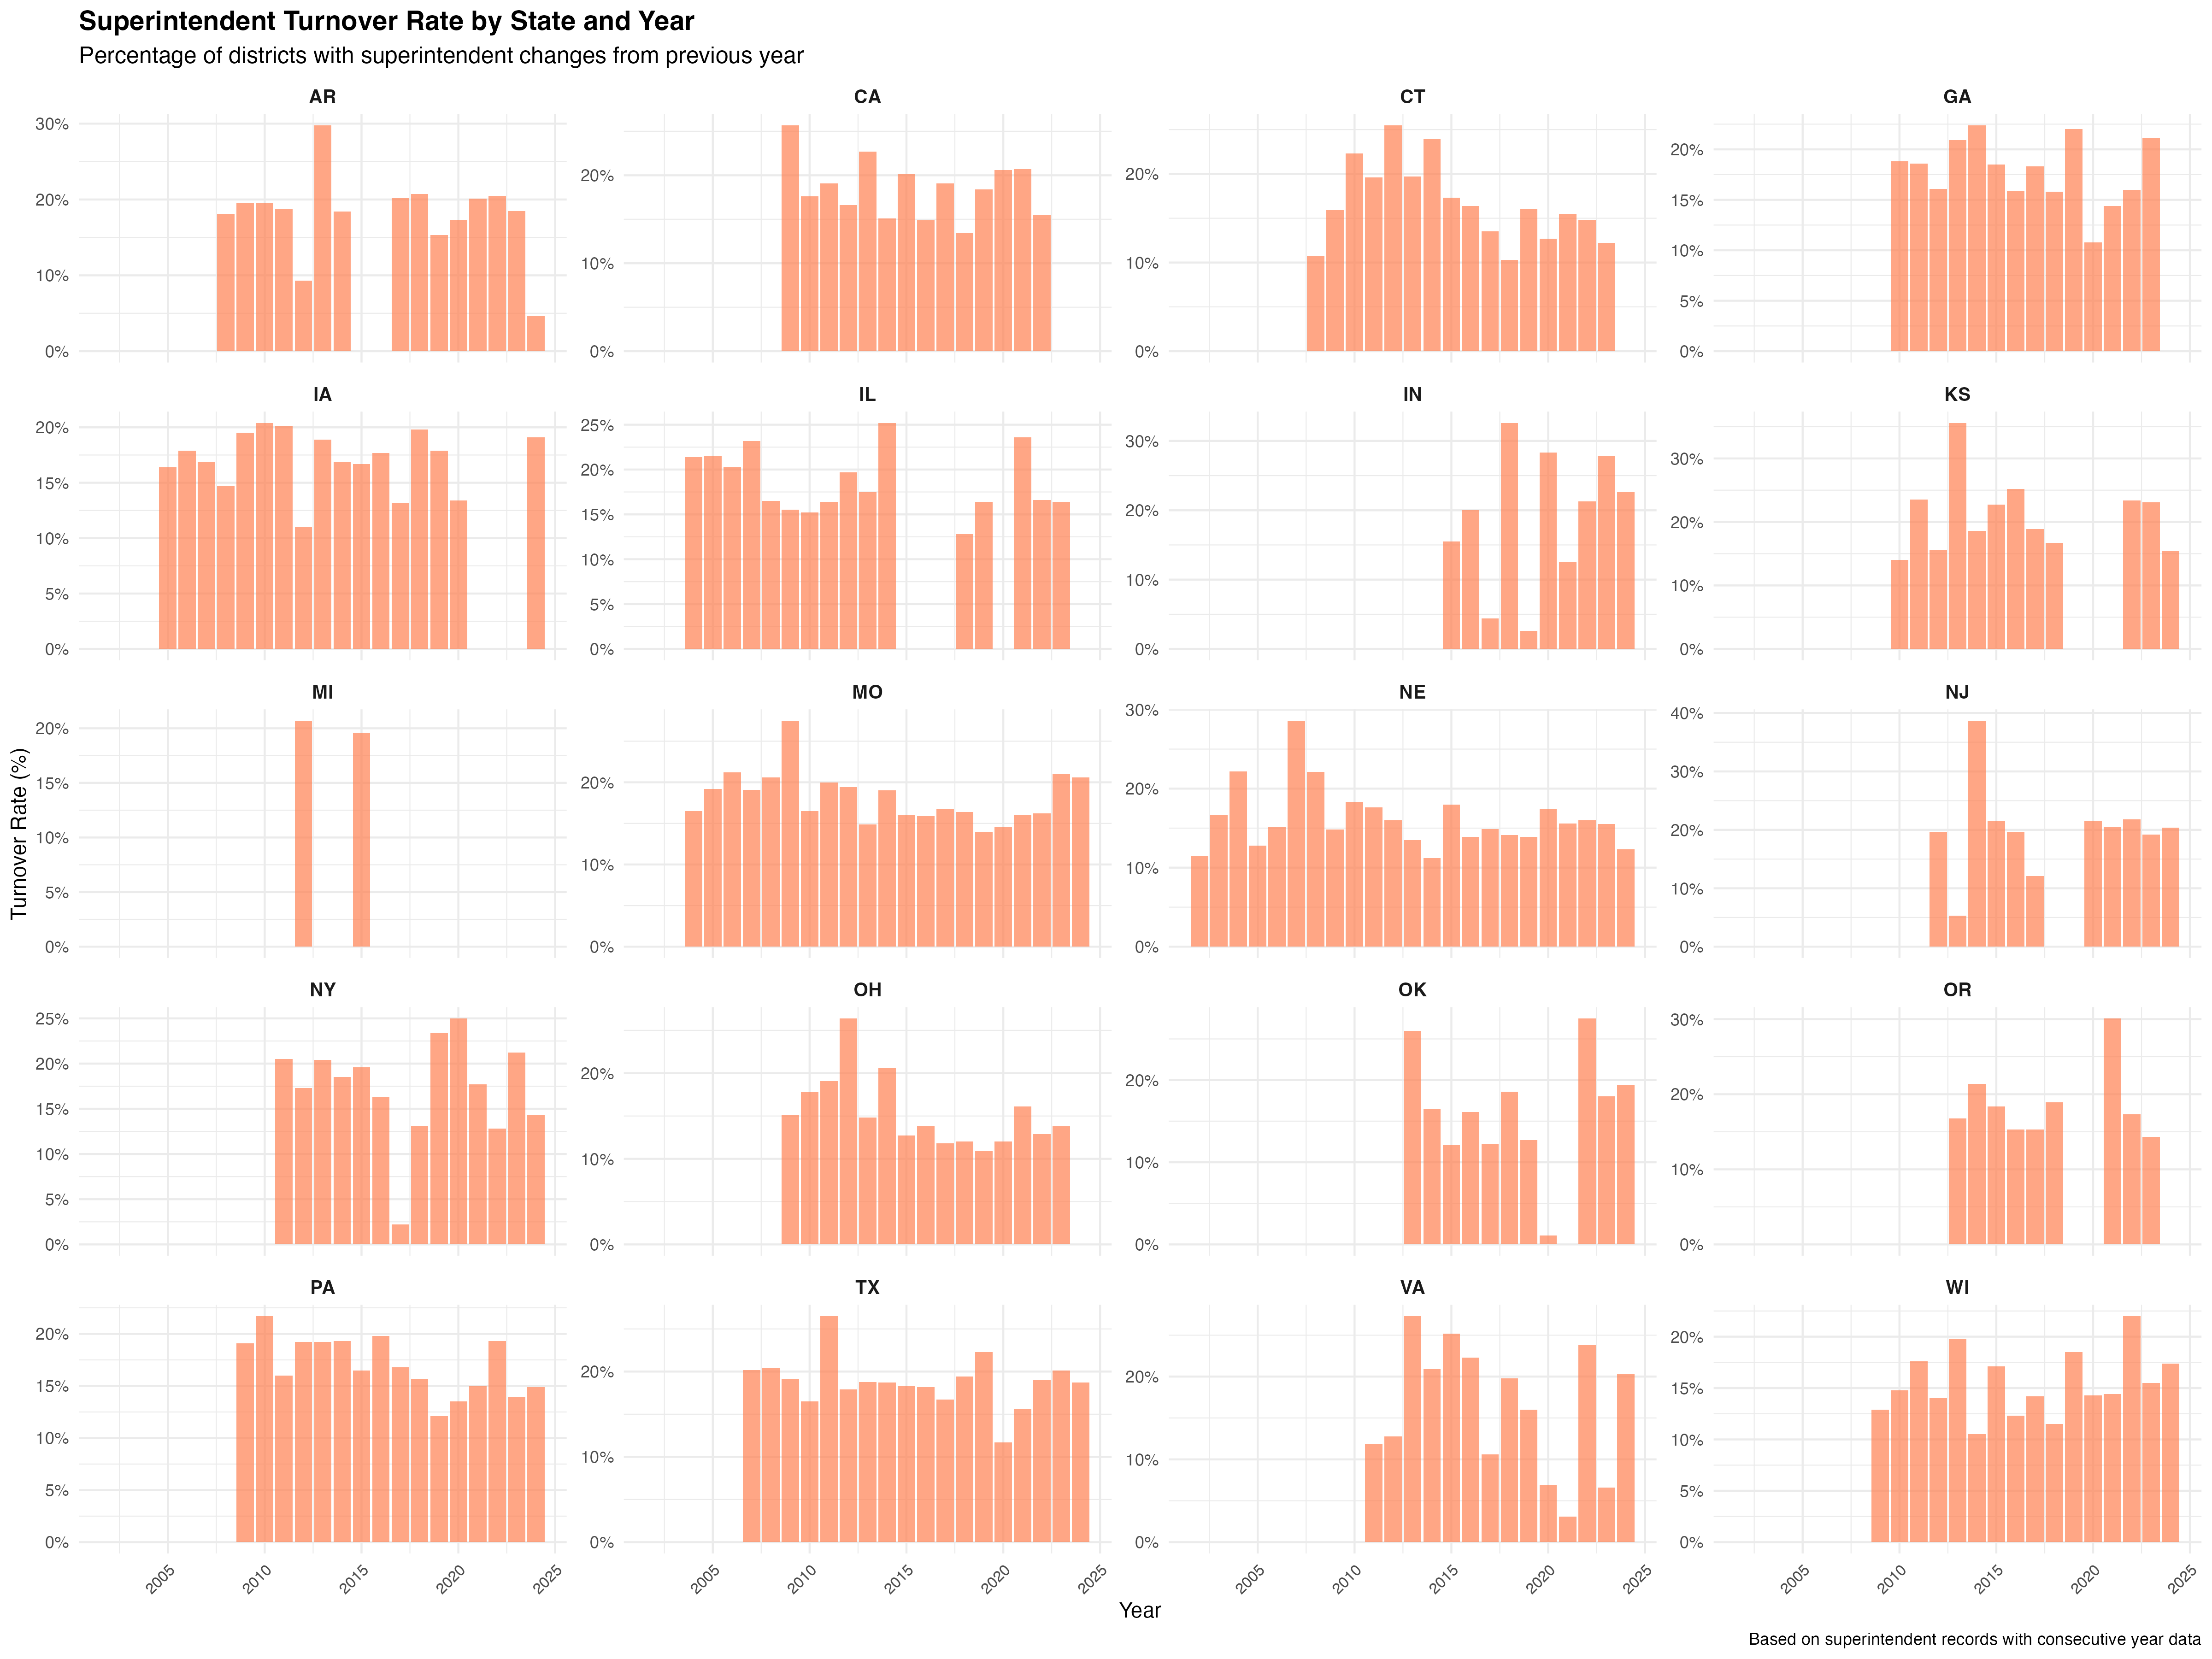
\includegraphics[width=0.9\textwidth]{figures/superintendent_turnover_by_state_year.png}
    \caption*{\footnotesize Notes: A district is considered to have a superintendent turnover if the superintendent name in a district changes from one year to the next. We use a string similarity score to allow for minor changes in name spelling or formatting across years. The turnover status for a given district and year is set to missing if the previous year's data is not available for that district. }
\end{figure}


\section*{Tables}
\begin{table}[H]
    \caption{Enrollment and district coverage, 2014}
    \label{tab:superintendent_coverage_enrollment_2014}
    \centering
    
\begin{tabular}{ccccc}
\toprule
State & Total Enrollment & Enrollment Coverage (\%) & Total Districts & District Coverage (\%)\\
\midrule
AR & 479,027 & 100 & 237 & 99.2\\
CA & 6,156,897 & 100 & 992 & 99.2\\
CT & 509,248 & 97.8 & 170 & 94.7\\
GA & 1,717,805 & 100 & 180 & 100\\
IA & 505,311 & 100 & 346 & 97.7\\
\addlinespace
IL & 2,046,476 & 99.9 & 862 & 98.3\\
IN & 1,004,622 & 100 & 291 & 99.7\\
KS & 496,920 & 100 & 307 & 93.2\\
MI & 1,350,667 & 100 & 543 & 100\\
MO & 897,427 & 93.6 & 520 & 91\\
\addlinespace
NE & 312,281 & 100 & 251 & 97.6\\
NJ & 1,363,220 & 100 & 588 & 99.3\\
NY & 1,637,426 & 100 & 688 & 100\\
OH & 1,601,836 & 99.9 & 615 & 99\\
OK & 671,715 & 100 & 517 & 99.8\\
\addlinespace
OR & 566,951 & 100 & 181 & 98.9\\
PA & 1,589,440 & 99.9 & 501 & 99.4\\
TX & 5,003,912 & 80.3 & 1,026 & 77.6\\
VA & 1,265,944 & 98.4 & 130 & 97.7\\
WI & 860,784 & 99.4 & 422 & 98.6\\
\addlinespace
US & 47,489,409 & 61 & 13,080 & 68.8\\
\bottomrule
\end{tabular}

    \caption*{\footnotesize Notes: This table shows total enrollment and district counts by state and in our dataset in 2014. As in Figure 2, these calculations only include regular public school districts, as designated by the CCD. This figure is a replication of \cite{stemper} Table 1 (re-produced as Table 7 in this document).}
\end{table}


\begin{table}[H]
    \caption{Turnover: comparison to \citet{white}}
    \label{tab:white_turnover_table}
    \centering
    \centering
\begin{tabular}{lccc}
\toprule
State & 2020 (\%) & 2021 (\%) & 2022 (\%) \\
\midrule
AR & 17.3 & 20.1 & 20.5 \\
CA & 20.6 & 20.7 & 15.5 \\
CT & 12.7 & 15.5 & 14.8 \\
GA & 10.8 & 14.4 & 16.0 \\
IA & 13.4 & NA & NA \\
IL & 0.0 & 23.6 & 16.6 \\
IN & 28.3 & 12.6 & 21.3 \\
KS & NA & NA & 23.4 \\
MO & 14.6 & 16.0 & 16.2 \\
NE & 17.4 & 15.6 & 16.0 \\
NJ & 21.6 & 20.5 & 21.8 \\
NY & 25.0 & 17.7 & 12.8 \\
OH & 12.0 & 16.1 & 12.9 \\
OK & 1.1 & 0.0 & 27.5 \\
OR & NA & 30.1 & 17.3 \\
PA & 13.5 & 15.0 & 19.3 \\
TX & 11.7 & 15.6 & 19.0 \\
VA & 6.9 & 3.1 & 23.8 \\
WI & 14.3 & 14.4 & 22.0 \\
\midrule
Total & 14.1 & 16.6 & 18.3 \\
National & 14.2 & 16.9 & 17.1 \\
\bottomrule
\end{tabular}
\label{tab:turnover_rates}


    \caption*{\footnotesize Notes: A district is considered to have a superintendent turnover if the superintendent name in a district changes from one year to the next. We use a string similarity score to allow for minor changes in name spelling or formatting across years. The turnover status for a given district and year is set to missing if the previous year's data is not available for that district. Total turnover rates refer to the total for that year in our data. National turnover rates come from \citet{white} Appendix Table S2.}
\end{table}

\begin{table}[H]
    \caption{Share of male superintendents  (\%): comparison to \citet{superintendentlab} }
    \label{tab:superintendent_demographics}
    \centering
    
% Table created by stargazer v.5.2.3 by Marek Hlavac, Social Policy Institute. E-mail: marek.hlavac at gmail.com
% Date and time: Fri, Sep 05, 2025 - 12:12:37
% Requires LaTeX packages: dcolumn 
\begin{tabular}{@{\extracolsep{5pt}} D{.}{.}{-1} D{.}{.}{-1} D{.}{.}{-1} } 
\\[-1.8ex]\hline 
\hline \\[-1.8ex] 
\multicolumn{1}{c}{} & \multicolumn{1}{c}{The Broad Center (2023-24)} & \multicolumn{1}{c}{Sup. Lab (2024-25)} \\ 
\hline \\[-1.8ex] 
\multicolumn{1}{c}{AR} & 69.4 & 62.9 \\ 
\multicolumn{1}{c}{CT} & 64.6 & 71.4 \\ 
\multicolumn{1}{c}{GA} & 70.1 & 86.9 \\ 
\multicolumn{1}{c}{IA} & 85.5 & 71.8 \\ 
\multicolumn{1}{c}{IL} & 69.2 & 79.3 \\ 
\multicolumn{1}{c}{IN} & 66.4 & 80.5 \\ 
\multicolumn{1}{c}{KS} & 74.5 & 75.3 \\ 
\multicolumn{1}{c}{MO} & 73 & 67.1 \\ 
\multicolumn{1}{c}{NE} & 87 & 85.8 \\ 
\multicolumn{1}{c}{NJ} & 65.6 & 65.6 \\ 
\multicolumn{1}{c}{NY} & 70.7 & 71 \\ 
\multicolumn{1}{c}{OH} & 81.3 & 83.1 \\ 
\multicolumn{1}{c}{OK} & 73.7 & 78.7 \\ 
\multicolumn{1}{c}{OR} & 63.9 & 67.3 \\ 
\multicolumn{1}{c}{PA} & 75.2 & 75 \\ 
\multicolumn{1}{c}{TX} & 68.4 & 74.6 \\ 
\multicolumn{1}{c}{VA} & 62.5 & 64 \\ 
\multicolumn{1}{c}{WI} & 72.7 & 74.8 \\ 
\multicolumn{1}{c}{Total} & 71.9 & 72.5 \\ 
\hline \\[-1.8ex] 
\end{tabular} 
\\
    \raggedright \footnotesize Notes: Gender is predicted based on the superintendent name using the \textbf{gender} package in R.\\ The right column is from \cite{superintendentlab}.
\end{table}

\newpage
\printbibliography

\end{document}


